%% TITLE	Physiological Fluid Mechanics, Summary 2

%% DATE		- May 17, 2022     first release
%%          - Nov 19, 2023      update

%% AUTHOR	BINGHUAN W LI (Dept. Chemical Eng/Bio Eng, Imperial)
%%          PETER Y XIE (Dept. Mech Eng, Stanford)

%% compiled in XeLaTeX with Tex Live version 2023.

%% This work is licensed under a Creative Commons Attribution-NonCommercial 4.0 International License.

\documentclass[a4paper]{article}
\newcommand{\summaryNo}{2}
%% TITLE	Physiological Fluid Mechanics, configuration

%% DATE		- Nov 19, 2023     create

%% AUTHOR	BINGHUAN W LI (Dept. Chemical Eng/Bio Eng, Imperial)
%%          PETER Y XIE (Dept. Mech Eng, Stanford)

%% compiled in XeLaTeX with Tex Live version 2023.

%% This work is licensed under a Creative Commons Attribution-NonCommercial 4.0 International License.

\usepackage[sfdefault]{arimo}
\usepackage[left=1.5cm, right=1.5cm, top=2cm, bottom=1.5cm]{geometry}
\usepackage{amsmath, amsfonts, amssymb, cancel}
\usepackage{unicode-math}
\setmathfont
    [    Extension = .otf,
         BoldFont = XITSMath-Bold,
    ]{XITSMath-Regular}

% % \DeclareMathSizes{10}{12}{10}{9}

% \usepackage{siunitx}
\usepackage{enumitem}
\usepackage{xcolor}
    \definecolor{linkcolour}{rgb}{0,0.2,0.6}
\usepackage{hyperref}
\hypersetup{
    colorlinks,
    breaklinks,
    urlcolor=linkcolour,
    linkcolor=linkcolour,
    citecolor=black,
    pdfauthor={Li, Binghuan W},
    }
\usepackage{graphicx, float}
\usepackage{framed}
\usepackage[export]{adjustbox}

\usepackage{fancyhdr}
    \pagestyle{fancy}
    \fancyhf{}
    \lhead{\textsc{Physiological Fluid Mechanics Summary \summaryNo}}
    \rhead{page \thepage}

\usepackage{tcolorbox}

\usepackage{tikz, circuitikz}

\usepackage{multicol}
    \setlength{\columnseprule}{1pt}

\usepackage{lscape}

\usepackage{booktabs}

\usepackage{pifont}

\setlength\parindent{0pt}

\begin{document}

\section{Conservation Principles}
\paragraph{Conservation of Momentum (Navier-Stokes)}
    \[
        \rho \bigg( \underbrace{\frac{\partial u_{i}}{\partial t}}_{\text{\ding{192}}} + \underbrace{u_{j}\frac{\partial u_{i}}{\partial x_{j}}}_{\text{\ding{193}}} \bigg) = -\underbrace{\frac{\partial p}{\partial x_{i}}}_{\text{\ding{194}}} + \underbrace{\mu \frac{\partial u_{i}}{\partial x_{j}\partial x_{j}}}_{\text{\ding{195}}} + \underbrace{\rho f_{i}}_{\text{\ding{196}}}
    \]
    \begin{center}
    \begin{tabular}{llll}
        \text{\ding{192}} & rate of change of speed (unsteady)&
        \text{\ding{193}} & convective acceleration \\
        \text{\ding{194}} & pressure gradient  &
        \text{\ding{195}} & diffusion (viscous) acceleration \\
        \text{\ding{196}} & body force \\
    \end{tabular}
    \end{center}
    Non-linearity due to the presence of the convective acceleration term, hence, the N-S cannot be decomposed using basis functions (\textit{e.g.} Fourier series).
        
\paragraph{Conservation of Energy}
    \[
        \rho c_{v} \bigg( \underbrace{\frac{\partial T}{\partial t}}_{\text{\ding{192}}} +\underbrace{\mathbf{u}\cdot \nabla T}_{\text{\ding{193}}} \bigg) = \underbrace{k\nabla^{2}T}_{\text{\ding{194}}} + \underbrace{\Phi}_{\text{\ding{195}}} + \underbrace{\dot{S}}_{\text{\ding{196}}} 
    \]
    \begin{center}
    \begin{tabular}{llll}
        \text{\ding{192}} & rate of change of heat &
        \text{\ding{193}} & heat convection \\
        \text{\ding{194}} & Heat conduction  &
        \text{\ding{195}} & work done by fluid shear and pressure \\
        \text{\ding{196}} & energy production \\
    \end{tabular}
    \end{center}

\paragraph{Conservation of Mass}
\[
    \frac{\partial C}{\partial t} + (\mathbf{u} \cdot \nabla)C = \mathcal{D}\nabla^2 C + \dot{S}_{v}
\]

\section{The Navier-Stokes Equations}
    \paragraph{Cartesian Coordinates} 
        \begin{itemize}
            \item Continuity Equation:
            \[\frac{\partial u}{\partial x} + \frac{\partial v}{\partial y} + \frac{\partial w}{\partial z}=0\]
            
            \item Momentum Equations:
            \[x: \ \rho \bigg(\frac{\partial u}{\partial t} + u \frac{\partial u}{\partial x} + v\frac{\partial u}{\partial y} + w\frac{\partial u}{\partial z} \bigg) = -\frac{\partial p}{\partial x} + \mu \bigg(\frac{\partial^{2} u}{\partial x^{2}} + \frac{\partial^{2} u}{\partial y^{2}} + \frac{\partial^{2} u}{\partial z^{2}}\bigg) + \rho f_{x}\]
            
            \[y: \ \rho \bigg(\frac{\partial v}{\partial t} + u \frac{\partial v}{\partial x} + v\frac{\partial v}{\partial y} + w\frac{\partial v}{\partial z} \bigg) = -\frac{\partial p}{\partial y} + \mu \bigg(\frac{\partial^{2} v}{\partial x^{2}} + \frac{\partial^{2} v}{\partial y^{2}} + \frac{\partial^{2} v}{\partial z^{2}}\bigg) + \rho f_{y}\]
            
            \[z: \ \rho \bigg(\frac{\partial w}{\partial t} + u \frac{\partial w}{\partial x} + v\frac{\partial w}{\partial y} + w\frac{\partial w}{\partial z} \bigg) = -\frac{\partial p}{\partial z} + \mu \bigg(\frac{\partial^{2} w}{\partial x^{2}} + \frac{\partial^{2} w}{\partial y^{2}} + \frac{\partial^{2} w}{\partial z^{2}}\bigg) + \rho f_{z}\]
            
        \end{itemize}
    
    \paragraph{Cylindrical Coordinates} 
        \begin{itemize}
            \item Continuity Equation:
            \[\frac{1}{r}\frac{\partial ru_{r}}{\partial r} + \frac{1}{r}\frac{\partial u_{\theta}}{\partial \theta} + \frac{\partial u_{z}}{\partial z}=0\]
            
            \item Momentum Equations:
            
            \[r: \ \rho \bigg(\frac{\partial u_{r}}{\partial t} + u_{r} \frac{\partial u_{r}}{\partial r} + \frac{u_{\theta}}{r}\frac{\partial u_{r}}{\partial \theta} + u_{z}\frac{\partial u_{r}}{\partial z} - \frac{u_{\theta}^{2}}{r} \bigg) = -\frac{\partial p}{\partial r} + \mu \bigg[ \frac{1}{r}\frac{\partial}{\partial r} \bigg(r \frac{\partial u_{r}}{\partial r}\bigg) + \frac{1}{r^{2}} \frac{\partial^{2} u_{r}}{\partial \theta^{2}} + \frac{\partial^{2} u_{r}}{\partial z^{2}} - \frac{u_{r}}{r^{2}} - \frac{2}{r^{2}}\frac{\partial u_{\theta}}{\partial \theta}\bigg] + \rho f_{r}\]
            
            \[\theta: \ \rho \bigg(\frac{\partial u_{\theta}}{\partial t} + u_{r} \frac{\partial u_{\theta}}{\partial r} + \frac{u_{\theta}}{r} \frac{\partial u_{\theta}}{\partial \theta} + u_{z}\frac{\partial u_{\theta}}{\partial z} + \frac{u_{r}u_{\theta}}{r} \bigg) = -\frac{1}{r} \frac{\partial p}{\partial \theta} + \mu \bigg[ \frac{1}{r}\frac{\partial}{\partial r} \bigg(r \frac{\partial u_{\theta}}{\partial r}\bigg) + \frac{1}{r^{2}} \frac{\partial^{2} u_{\theta}}{\partial \theta^{2}} + \frac{\partial^{2} u_{\theta}}{\partial z^{2}} - \frac{u_{\theta}}{r^{2}} + \frac{2}{r^{2}}\frac{\partial u_{r}}{\partial \theta}\bigg] + \rho f_{\theta}\]
            
            \[z: \ \rho \bigg(\frac{\partial u_{z}}{\partial t} + u_{r} \frac{\partial u_{z}}{\partial r} + \frac{u_{\theta}}{r}\frac{\partial u_{z}}{\partial \theta} + u_{z}\frac{\partial u_{z}}{\partial z} \bigg) = -\frac{\partial p}{\partial z} + \mu \bigg[ \frac{1}{r}\frac{\partial}{\partial r} \bigg(r \frac{\partial u_{z}}{\partial r}\bigg) + \frac{1}{r^{2}} \frac{\partial^{2} u_{z}}{\partial \theta^{2}} + \frac{\partial^{2} u_{z}}{\partial z^{2}} \bigg] + \rho f_{z}\]
        \end{itemize}
    
    \paragraph{Spherical Coordinates}
        \begin{itemize}
            \item Continuity Equation:
            \[\frac{1}{r^{2}}\frac{\partial r^{2}u_{r}}{\partial r} + \frac{1}{r \sin \theta}\frac{\partial u_{\theta}\sin \theta}{\partial \theta} + \frac{1}{r \sin \theta}\frac{\partial u_{\phi}}{\partial \phi}=0\]
            
            \item Momentum Equations:
            
            \begin{equation*}
            \begin{split}
            r: \ & \rho \bigg(\frac{\partial u_{r}}{\partial t} + u_{r} \frac{\partial u_{r}}{\partial r} + \frac{u_{\theta}}{r}\frac{\partial u_{r}}{\partial \theta} + \frac{u_{\phi}}{r \sin \theta} \frac{\partial u_{r}}{\partial \phi} - \frac{u_{\theta}^{2}+u_{\phi}^{2}}{r} \bigg)  \\ 
            & = -\frac{\partial p}{\partial r} + \mu \bigg( \nabla^{2}u_{r} - \frac{2u_{r}}{r^{2}} - \frac{2}{r^{2}\sin \theta}\frac{\partial}{\partial \theta}(u_{\theta}\sin\theta) + \frac{2}{r^{2}\sin\theta}\frac{\partial u_{\phi}}{\partial \phi} \bigg) + \rho f_{r}
            \end{split}  
            \end{equation*}
            
            \begin{equation*}
            \begin{split}
            \theta: \ & \rho \bigg(\frac{\partial u_{\theta}}{\partial t} + u_{r} \frac{\partial u_{\theta}}{\partial r} + \frac{u_{\theta}}{r} \frac{\partial u_{\theta}}{\partial \theta} + \frac{u_{\phi}}{r\sin \theta} \frac{\partial u_{\theta}}{\partial \phi} + \frac{u_{r}u_{\theta}-u_{\phi}^{2}\cot\theta}{r} \bigg) \\
            & = -\frac{1}{r}\frac{\partial p}{\partial \theta} + \mu \bigg( \nabla^{2}u_{\theta} - \frac{u_{\theta}}{r^{2}\sin^{2}\theta} + \frac{2}{r^{2}}\frac{\partial u_{r}}{\partial \theta} - \frac{2\cos \theta}{r^{2}\sin^{2}\theta}\frac{\partial u_{\phi}}{\partial \phi} \bigg) + \rho f_{\theta}
            \end{split}  
            \end{equation*}
            
            \begin{equation*}
            \begin{split}
            \phi: \ & \rho \bigg(\frac{\partial u_{\phi}}{\partial t} + u_{r} \frac{\partial u_{\phi}}{\partial r} + \frac{u_{\theta}}{r} \frac{\partial u_{\phi}}{\partial \theta} + \frac{u_{\phi}}{r\sin \theta} \frac{\partial u_{\phi}}{\partial \phi} + \frac{u_{r}u_{\phi}+u_{\phi}u_{\theta}\cot\theta}{r} \bigg) \\
            & = -\frac{1}{r\sin\theta}\frac{\partial p}{\partial \phi} + \mu \bigg( \nabla^{2}u_{\phi} - \frac{u_{\phi}}{r^{2}\sin^{2}\theta} + \frac{2}{r^{2}\sin \theta}\frac{\partial u_{r}}{\partial \phi} - \frac{2\cos \theta}{r^{2}\sin^{2}\theta}\frac{\partial u_{\theta}}{\partial \phi} \bigg) + \rho f_{\phi}
            \end{split}  
            \end{equation*}
        \end{itemize}

    \subsection{Assumptions with Navier-Stokes Equations}
    \begin{multicols}{2}
    \begin{itemize}
        \item Steady flow: $\displaystyle \frac{\partial}{\partial t} = 0$
        
        \item Fully developed flow (in $z$-direction): $\displaystyle \frac{\partial}{\partial z} = 0$
        
        \item Axisymmetric flow  (in cylindrical coord.): $\displaystyle \frac{\partial}{\partial \theta} = 0$
        
        \item Spherical symmetric flow: $\displaystyle \frac{\partial}{\partial \theta} = 0, \frac{\partial}{\partial \phi} = 0$
        
        \item No Swirl: $u_{\theta} = 0$
        
        \item Two-dimensional flow (with $z$-direction absent): $\displaystyle u_{z}=0$ and $\displaystyle \frac{\partial}{\partial z} = 0$
    \end{itemize}
    \end{multicols}
    
\vfill
{\small \color{gray}Drafted by B. Li, \today}
\thispagestyle{empty}
\newgeometry{margin=1.8cm}
\mbox{}
\vfill    
\begin{figure}[H]
    \includegraphics[right]{images/by-nc.eps}
\end{figure}
\textit{This work is licensed under a Creative Commons Attribution-NonCommercial 4.0 International License.}


\end{document}